\documentclass[../paper.tex]{subfiles}
\usepackage{graphicx} % Required for inserting images
\graphicspath{{\subfix{../Figures/}}}

\usepackage{amssymb}
\usepackage{amsmath}
\usepackage{amsthm}
\usepackage{mathtools}
\usepackage{hyperref}

\usepackage{biblatex} %Imports biblatex package
\addbibresource{references.bib} %Import the bibliography file

\usepackage{xcolor}

\usepackage{comment}

\begin{document}

We present a novel method to analytically evaluate our integrals on triangles that works for all cases except for when the target point $\x$ 
lies inside the triangle $\Delta$ when integrating $K(\x, \y)p(\y)$. This is done by using a polar coordinate transform that greatly simplifies the integrand. Once in the new polar coordinate system, we give an algorithm that finds the bounds on integration that then gives explicit closed form formulas for the integral. 

As $\x$ becomes closer to $\Delta$, the numerical integral starts to blow up, making it ``near-singular''. Adaptive refinement of the triangles can give very accurate results in the near-singular case \cite{atkinson1997numerical}, but also greatly increases algorithm runtime. 

Other papers have also tried to give analytic formulas, but either their formulas require special assumptions or need to split the triangle into special sub-triangles \cite{carley2013analytical, okon1982potentialLinear, bohm2024efficient}. \cite{graglia1993numerical} gives very similar polar transforms as we do for near singular integrals, but we argue that our new algorithm for determining bounds on integration allows for more generalization. 
We consider the general case of evaluating \autoref{eq: general integral problem gradient green} on any arbitrary triangle $\Delta$. 

\subsection{Choosing the correct polar coordinates}
To obtain an analytic solution to our integral on a triangle, we use polar coordinates and a transformation that allows us to invoke Pythagoras' theorem. 
Our transformations needs to preserve Euclidean distance, so it can only be a combinations of rotations and translations.
We map $\Delta$ to a triangle $\Delta_{XY}$ that lies on the $XY$-plane, such that the point $\x$ we are integrating it against lies on the $Z$-axis. 
This map is the rotational map between the triangle normal and the vector $[0, 0, 1]$, followed by a translation. 
Let $n(\Delta)$ be the normal vector of the arbitrary triangle. We want to find a map that rotates $n(\Delta)$ into $[0, 0, 1]^T$, the normal vector of a triangle that lies on the $XY$-plane. 
This rotational map $R$ is the $3\times 3$ matrix defined by 
\begin{equation}
    R = \cos(\alpha)I +(1-\cos(\alpha))* s^T s + \sin(\alpha) * [v]_{\times} 
\end{equation}
where we define
\begin{equation*}
    v = n(\Delta) \times \begin{bmatrix}
        0\\
        0\\
        1\\
    \end{bmatrix}, \quad \alpha = \arccos\left(n(\Delta) \cdot \begin{bmatrix} 
        0\\
        0\\
        1\\
    \end{bmatrix}\right), \quad s = \frac{v}{\|v\|}
\end{equation*}
and $[v]_{\times}$ is the skew symmetric matrix of $v= \begin{bmatrix}
    v_1 \\
    v_2 \\
    v_3 \\
\end{bmatrix}$ defined by 
\begin{equation}
    [v]_{\times} = \begin{bmatrix}
        0 & -v_3 & v_2\\
        v_3 & 0 & -v_1\\
        -v_2 & v_1 & 0\\
    \end{bmatrix}.
\end{equation}
This is commonly known as Rodrigues' rotation formula.
After applying the rotation, a translation is done to map the triangle onto the $XY$-plane and the point $R(\x)$ onto the $Z$-axis. 

As $\x$ lies on the $Z$-axis, we can write $\x = [0, 0, c]^T$. 
Pythagoras' theorem then gives $|\x - \y|^2 = y_x^2 + y_y^2 + c^2$, so the desired integral is 
\begin{equation*}
    I = \int_{\Delta_{XY}} \frac{-y_xn_x-y_yn_y+cn_z}{(y_x^2+y_y^2+c^2)^{3/2}} p(\y)\, dS_{\y}.
\end{equation*}
Assuming that the polynomial $p$ has degree at most 1, we simply need to compute the integrals  
\begin{align*}
I_0:=\int_\Delta \frac{1}{(y_x^2+y_y^2+c^2)^{3/2}} ~dS_{\y},~ I_x:=\int_\Delta \frac{y_x}{(y_x^2+y_y^2+c^2)^{3/2}}~dS_{\y}, \\ 
I_y:=\int_\Delta \frac{y_y}{(y_x^2+y_y^2+c^2)^{3/2}}~dS_{\y}, I_{x^2}:=\int_\Delta \frac{y_x^2}{(y_x^2+y_y^2+c^2)^{3/2}}~dS_{\y}, \\
I_{y^2}:=\int_\Delta \frac{y_y^2}{(y_x^2+y_y^2+c^2)^{3/2}}~dS_{\y},~ I_{xy}:=\int_\Delta \frac{y_xy_y}{(y_x^2+y_y^2+c^2)^{3/2}}~dS_{\y}.
\end{align*}
For example, if we consider $p(\y) = 1$, then the desired integral is 
\begin{align*}
I =  cn_z I_0 - n_x I_x - n_y I_y
\end{align*}

Introducing polar coordinates for $\y$: $y_x=r\cos\theta,~ y_y=r\sin\theta$, we can rewrite the integrals into the form
\begin{equation*}
    \int_{r_\mathrm{start}}^{r_\mathrm{end}} \int_{\theta_\mathrm{start}(r)}^{\theta_\mathrm{end}(r)} \frac{r^{a+b+1}(\cos(\theta))^a(\sin(\theta))^b}{(r^2+c^2)^{3/2}} ~d\theta dr
\end{equation*}
for powers $(a,b)$ that represents the powers of $y_x$ and $y_y$ in the numerator.  
The method to determine the values of $\theta_\mathrm{start}(r)$ and $\theta_\mathrm{end}(r)$ are explained in the following subsection.

\subsection{Determining start and end angles}
When we integrate in polar coordinates starting at the point $\y$ where the circle of radius $r$ intersects an edge of the triangle, 
the angle $\theta(r)$ of the point $\y$ can be written as 
\begin{equation}
    \theta_\mathrm{start}(r) = \arccos\left(\frac{y_x}{r}\right)
\end{equation}
However, $y_x$ is non-linearly dependent on $r$, so this does not give rise to a simple analytic solution. 
Instead, we look at the projection of the origin to the lines which define the sides of the triangle. 
Let us label the positively oriented vertices as $V_1, V_2, V_3$. 
Let $d_1$ be the projection of the origin to the line on which $V_1$ and $V_2$ lie on; $d_2$ be the projection of the origin to the line on which $V_2$ and $V_3$ lie on; 
and $d_3$ be the projection of the origin to the line on which $V_3$ and $V_1$ lie on.

Let $\phi_k$ be the angle between $d_k$ and the $X$-axis, then the angle at a point of intersection between a circle of radius $r$ and a side of the triangle is 

\begin{equation}\label{equation for boundary theta}
    \theta(r) = \pm\arccos\left(\frac{d_k}{r}\right) + \phi_k
\end{equation}
where $d_k$ is the orthogonal projection of the origin onto the line on which that specific edge of the triangle lies on. An example is shown in \autoref{fig:variablediagram}. 
The importance of this equation is that now 
\begin{equation*}
    \theta_\mathrm{start}(r) = \mathrm{sign}_\mathrm{start}\arccos\left(\frac{d_\mathrm{start}}{r}\right) + \phi_\mathrm{start} 
\end{equation*}
where $\mathrm{sign}_\mathrm{start}, d_\mathrm{start}, \phi_\mathrm{start}$ are all piece-wise constant in $r$. 
If we split our integral into the correct regions in $r$, it is much simpler to write out an analytic solution to our integral. 

\begin{figure}
\begin{center}
\begin{tikzpicture}

% draw the axes
\coordinate (xaxis) at (4.5,0);
\coordinate (yaxis) at (0,3.5);
\draw[->] (0,0) -- (xaxis) node[right] {$x$};
\draw[->] (0,0) -- (yaxis) node[above] {$y$};

% draw the triangle
\coordinate (V1) at (1.0,1.5);
\coordinate (V2) at (4.0,2.5);
\coordinate (V3) at (1.5,3.0);
\coordinate (dP12) at ( 3.0, 1.0);
\coordinate (dP23) at (-2.5, 0.5);
\coordinate (dP31) at (-0.5,-1.5);
\coordinate (P12r) at (-2,0.5);
\draw[fill=blue!20,opacity=0.5] (V1) -- (V2) -- (V3) -- cycle;

% label the vertices of the triangle
\node at (V1) [above left] {$\boldsymbol{V}_1$};
\node at (V2) [above] {$\boldsymbol{V}_2$};
\node at (V3) [above] {$\boldsymbol{V}_3$};
\fill (V1) circle (2pt);
\fill (V2) circle (2pt);
\fill (V3) circle (2pt);

% draw the intersections
\def\lval{3.0}; % radius length
\coordinate (L12) at (2.2953,1.9318);
\coordinate (L13) at (1.3867,2.6602);
\fill (L12) circle (1pt);
\fill (L13) circle (1pt);
\node at (L12) [left] {};
\node at (L13) [left] {};

% draw the integration path
\coordinate (O) at (0,0);
\fill (O) circle (2pt);
\draw[thick] (L12) arc (40.0847:62.4676:\lval);    
\draw[] (O) -- ++(0.6256*\lval,0.7802*\lval) node[below] {$r$};
\draw[] (O) -- (L12);
\draw[] (O) -- (L13);

% draw projections
\coordinate (Q12) at (-0.3500, 1.0500);
\coordinate (Q23) at ( 0.6346, 3.1731);
\coordinate (Q31) at ( 0.4500,-0.1500);

\fill (Q12) circle (2pt);
\draw[dashed] (O) -- ++(Q12) node[midway, left] {$d_{1}$};
\draw[dashed] (P12r) -- (Q12) -- (V1);
\pic [draw,below right, ->, "$~\phi_{1}$", angle eccentricity=1.0, angle radius=15] {angle = xaxis--O--Q12};
\pic [draw,right, ->, "$\theta_{12}(r)$", angle eccentricity=1.0, angle radius=50] {angle = xaxis--O--L12};

\pic [draw,above left, <-, "$\arccos(d_{1}/r)~~$", angle eccentricity=1.2, angle radius=28] {angle = L12--O--Q12};

%\fill (Q23) circle (1pt);
%\draw[dashed] (O) -- ++(Q23) node[midway, left] {$d_{23}$};
%\draw[dashed,opacity=0.5] (Q23) -- (P3);

%\fill (Q31) circle (1pt);
%\draw[dashed] (O) -- ++(Q31) node[midway, below] {$d_{31}$};
%\draw[dashed,opacity=0.5] (Q31) -- (P1);

\end{tikzpicture}
\end{center}
\caption{A diagram defining variables for the integration. The triangle $\Delta$ is defined by the points $V_1, V_2, V_3$. 
The distance from the origin to the projection of the origin onto the side $\overline{V_1V_2}$ is $d_{1}$; this projection makes an angle of $\phi_{1}$ with the $X$-axis. 
A circle of radius $r$ centered at the origin intersects the side $\overline{V_1V_2}$ with an angle of $\theta_{12}(r)$ with the $X$-axis. 
Similarly, this circle intersects side $\overline{V_3V_1}$ with an angle of $\theta_{31}(r)$ with the $X$-axis.\label{fig:variablediagram}}
\end{figure}

The critical radii $R_i$ which separates the regions on which $\mathrm{sign}_\mathrm{start}, d_\mathrm{start}, \phi_\mathrm{start}$ (and the corresponding end values) are constant are the norm of the three vertices of the triangle 
and the norm of the orthogonal projections $d_k$ if they lie on the triangle, ordered from smallest to largest. 
Starting at $r = 0$, the $\theta$ integral is either on $[0, 2\pi]$ or on $\emptyset$, depending on if the origin is in the triangle. 
This is easily checked numerically. Now as we progress through the different critical radii, we need to keep track on which angles we start and stop the integration. 
This is done by labeling the triangle edges and keeping track of their activity. 

\begin{definition}
    For a given radius $r$, the edge $\overline{V_1V_2}$ of a triangle with vertices $V_1, V_2, V_3$ lying on the $XY$-plane is \textbf{inactive} if the circle of radius $r$ on the $XY$ plane does not intersect $\overline{V_1V_2}$. 
    It is \textbf{active} if the circle of radius $r$ intersects it only once, and \textbf{split} if it intersects it twice. 
\end{definition}
The reason for this definition is to know what angles we use in our integrals. 
For example, at $r=0$, all edges are inactive unless the origin is one of the vertices, in which case two edges are active and one is inactive. 
If two edges are active while the third is inactive, then we only need to consider two angles and which one of them is the start angle and which is the end angle. 

To make sure that we are always integrating in the correct direction, we need to first order the vertices of the triangle such that its vertices $V_1, V_2, V_3$ are positively oriented and $V_1$ is the vertex closest to the origin. 

\begin{definition}\label{def: left and right}
    For a triangle in the previously specified configuration, if the projection point $d_{1}$ lies on the interior of the edge $\overline{V_1V_2}$, it splits the edge into $\overline{V_1d_1}$ and $\overline{d_1V_2}$, 
    which we define as its \textbf{left} and \textbf{right} respectively. For other projection points, the left and right are defined so that everything is still positively oriented. 
    If the projection point does not lie on the edge, that entire edge is considered as both left and right for the sake of the algorithm. 
\end{definition}

Note that when a projection point lies on an edge of the triangle, its left and right corresponds to different signs for arc-cosine. 
It is not trivial to determine which has the positive sign and which has the negative sign, so it must be computed by testing which sign of arc-cosine the vertices of that edge use. 
If $d_1$ lies on $\overline{V_1V_2}$, the simplest way is to check if which sign makes $V_1 = \pm\arccos\left(\frac{d_1}{\|V_1\|}\right) + \phi_1$ true.
This configuration makes it so that we always integrate from edges $\overline{V_1V_2}$ to $\overline{V_2V_3}$ to $\overline{V_3V_1}$. 
In the case where an edge is split, we use Definition \ref{def: left and right} to know that we always integrate starting the the right side of the first active or split edge and then alternate between left and right of the following edges. 

As the radius $r$ increases, the activity of the edges change when $r$ equals to a critical radii. 
At $r=R_i$, the change in the activities is dependent on whether $R_i$ is the norm of a vertex or a projection point. 
If it is the norm of a vertex, the activities of the edges the vertex lie on changes. Inactive edges become active while active edges become inactive. 
A split edge on the other hand becomes active. There is a special case where two vertices have the exact same norm, which can cause a split edge to become inactive. 
However, due to floating point precision, we do not consider this case. If $R_i$ is the norm of a projection point, the only case that happens is the inactive edge that it lies on becomes split. 
An example of how the activities change is shown in \autoref{fig:regiondiagram}. For more details, check the comments in the code, which we outline other special cases. 

\begin{figure}
\begin{center}
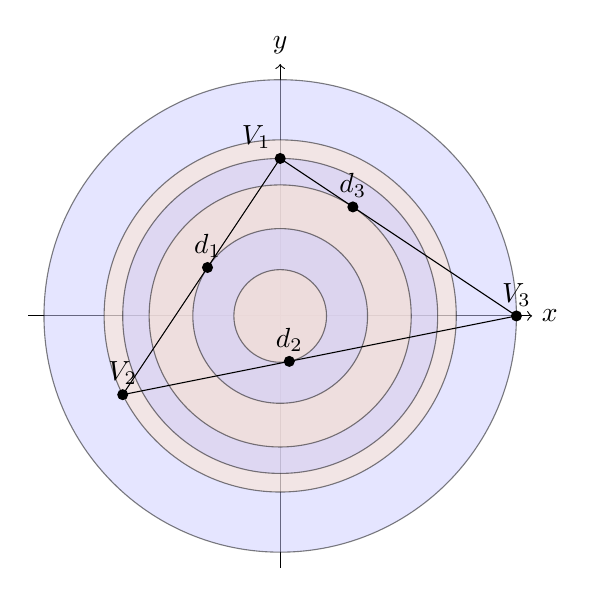
\begin{tikzpicture}

% draw the axes
\coordinate (xaxis) at (3.2,0);
\coordinate (yaxis) at (0,3.2);
\draw[->] (-3.2,0) -- (xaxis) node[right] {$x$};
\draw[->] (0,-3.2) -- (yaxis) node[above] {$y$};

% draw the triangle
\coordinate (V1) at (0, 2);
\coordinate (V2) at (-2, -1);
\coordinate (V3) at (3, 0);
\coordinate (dP12) at (-0.9231, 0.6154);
\coordinate (dP23) at (0.1154, -0.577);
\coordinate (dP31) at (0.923, 1.3846);

% give the critical radii
\def\rone{0.5883}; % radius length
\def\rtwo{1.1094}; % radius length
\def\rthree{1.6641}; % radius length
\def\rfour{2}; % radius length
\def\rfive{2.2361}; % radius length
\def\rsix{3}; % radius length

% draw the annulus
\draw[fill=blue!20, opacity=0.5] (0, 0) circle (\rsix);
\draw[fill=orange!20, opacity=0.5] (0, 0) circle (\rfive);
\draw[fill=blue!20, opacity=0.5] (0, 0) circle (\rfour);
\draw[fill=orange!20, opacity=0.5] (0, 0) circle (\rthree);
\draw[fill=blue!20, opacity=0.5] (0, 0) circle (\rtwo);
\draw[fill=orange!20, opacity=0.5] (0, 0) circle (\rone);

% label the vertices of the triangle
\node at (V1) [above left] {$V_1$};
\node at (V2) [above] {$V_2$};
\node at (V3) [above] {$V_3$};
\node at (dP12) [above] {$d_1$};
\node at (dP23) [above] {$d_2$};
\node at (dP31) [above] {$d_3$};
\fill (V1) circle (2pt);
\fill (V2) circle (2pt);
\fill (V3) circle (2pt);
\fill (dP12) circle (2pt);
\fill (dP23) circle (2pt);
\fill (dP31) circle (2pt);
\draw[] (V1) -- (V2) -- (V3) -- cycle;

\end{tikzpicture}
\end{center}
\caption{A diagram showing the different critical radii for integration. 
The triangle $\Delta$ is defined by the points $V_1, V_2, V_3$. 
The projection of the origin to the edges of the triangles are labeled with $d_1, d_2, d_3$, which in this case all lie on their respective edges. 
Letting $-1$ represent inactive, $1$ represent active, and $0$ represent split, the activities of the edges ordered in $[\overline{V_1V_2}, \overline{V_2V_3}, \overline{V_3V_1}]$ change as follows. 
Starting from $r=0$, $[-1, -1, -1]\rightarrow [-1, 0, -1] \rightarrow [0, 0, -1] \rightarrow [0, 0, 0] \rightarrow [1, 0, 1] \rightarrow [-1, 1, 1] \rightarrow [-1, -1, -1]$\label{fig:regiondiagram}}
\end{figure}

This algorithm can then be used to integrate any function on any triangle that lies on $\mathbb{R}^2$ without the need to apply some non-distance preserving transform. 

\subsection{Example}

Now that we can accurately determine the activity of each edge and which sign each arc-cosine has, we can integrate on the triangle. We denote
\begin{equation*}
\begin{split}
    \theta_{\mathrm{end}}(r) &= \mathrm{sign}_\mathrm{end}\arccos\left(\frac{d_\mathrm{end}}{r}\right) + \phi_\mathrm{end},\\
    \theta_{\mathrm{start}}(r) &= \mathrm{sign}_\mathrm{start}\arccos\left(\frac{d_\mathrm{start}}{r}\right) + \phi_\mathrm{start}.
\end{split}
\end{equation*}

The analytic formula for $I_0$ is 
\begin{equation*}
\begin{split}
    I_0  & = \int_{r_\mathrm{start}}^{r_\mathrm{end}} \int_{\phi_\mathrm{start} + \mathrm{sign}_\mathrm{start}\arccos\left(d_\mathrm{start}/r\right)}^{\phi_\mathrm{end} + \mathrm{sign}_\mathrm{end}\arccos\left(d_\mathrm{end}/r\right)} \frac{r}{(r^2 + c^2)^{3/2}}\, d\theta \, dr \\
    & = (\phi_\mathrm{start} - \phi_\mathrm{end}) \int_{r_\mathrm{start}}^{r_\mathrm{end}} \frac{r}{(r^2+c^2)^{3/2}}\, dr + \mathrm{sign}_\mathrm{end}\int_{r_\mathrm{start}}^{r_\mathrm{end}} \frac{r}{(r^2 + c^2)^{3/2}}\arccos\left(\frac{d_\mathrm{end}}{r}\right)\, dr \\
    & - \mathrm{sign}_\mathrm{start}\int_{r_\mathrm{start}}^{r_\mathrm{end}} \frac{r}{(r^2 + c^2)^{3/2}}\arccos\left(\frac{d_\mathrm{start}}{r}\right)\, dr \\
\end{split}
\end{equation*}
The three integrals in $r$ have analytic formulas which are found in Appendix \ref{appendix: formula for integral of normal derivative of single layer potential}. Other types of integrals once written in a similar form can also be evaluated by analytically evaluating the integrals in $r$ by hand or by using mathematical programs like Mathematica. 

Similar formulas are also obtained if we want to integrate \autoref{eq: general integral problem green}, and in this case the formulas also work for any arbitrary $\x$.

\end{document}

